\documentclass[a4paper]{article}
%\usepackage[singlespacing]{setspace}
\usepackage[onehalfspacing]{setspace}
%\usepackage[doublespacing]{setspace}
\usepackage{geometry} % Required for adjusting page dimensions and margins
\usepackage{amsmath,amsfonts,stmaryrd,amssymb,mathtools,dsfont} % Math packages
\usepackage{tabularx}
\usepackage{colortbl}
\usepackage{listings}
\usepackage{amsmath}
\usepackage{amssymb}
\usepackage{amsthm}
\usepackage{subcaption}
\usepackage{float}
\usepackage[table,xcdraw]{xcolor}
\usepackage{tikz-qtree}
\usepackage{changepage,titlesec,fancyhdr} % For styling Header and Titles
\pagestyle{fancy}
\usepackage{array}

\usepackage{enumerate} % Custom item numbers for enumerations

\usepackage[ruled]{algorithm2e} % Algorithms

\usepackage[framemethod=tikz]{mdframed} % Allows defining custom boxed/framed environments

\usepackage{listings} % File listings, with syntax highlighting
\lstset{
	basicstyle=\ttfamily, % Typeset listings in monospace font
}

\usepackage[ddmmyyyy]{datetime}


\geometry{
	paper=a4paper, % Paper size, change to letterpaper for US letter size
	top=2.5cm, % Top margin
	bottom=3cm, % Bottom margin
	left=2.5cm, % Left margin
	right=2.5cm, % Right margin
	headheight=25pt, % Header height
	footskip=1.5cm, % Space from the bottom margin to the baseline of the footer
	headsep=1cm, % Space from the top margin to the baseline of the header
	%showframe, % Uncomment to show how the type block is set on the page
}
\lhead{ALGO-1\\Sommersemester 2024}
\chead{\bfseries{Übungsblatt 5}\\}
\rhead{7987847\\Jonas Werner}

\begin{document}

\section*{Aufgabe 5.1}
Bestimmen Sie für jeden leeren Eintrag aus der folgenden Tabelle das richtige Verhältnis zwischen
$f$ und $g$. Eine Begründung ist nicht nötig.\\

\begin{tabular}{| c | c | c | c | c | c |}
  \hline
   & $g(n) = 3n$ & $g(n) = n \sqrt{n}$ & $g(n) = 1$ & $g(n) = log^2(n)$ & $g(n) = \binom{n}{2}$ \\
  \hline
  $f(n) = n^2$ & $g = o(f)$ & $g = o(f)$ & $g = o(f)$ & $g = o(f)$ & $g = \theta(f)$ \\
  \hline
  $f(n) = \sqrt{n}$ & $f = o(g)$ & $f = o(g)$ & $g = o(f)$ & $g = o(f)$ & $f = o(g)$ \\
  \hline
  $f(n) = log(log(n))$ & $f = o(g)$ & $f = o(g)$ & $g = o(f)$ & $f = o(g)$ & $f = o(g)$ \\
  \hline
\end{tabular}

\section*{Aufgabe 5.2}
\subsection*{a)}
\[ T(n) = T\left(\frac{n}{3}\right) + n\]

Daraus lassen sich folgende Werte ablesen:
\begin{itemize}
    \item $a = 1$
    \item $b = 3$
    \item $t(n) = n $
    \item $k = 1$
\end{itemize}

Damit berechnen wir:
\[ \log_b a = \log_3 1 = 0 < k = 1 \]

Daraus folgt:
\[
\Rightarrow \text{Es tritt Fall (c) ein.}
\]

Somit gilt die folgende Gleichung:
\[ T(n) = \theta\left(t(n)\right) = \theta\left(n\right)\]

\break

\subsection*{b)}
\[ T(n) = 2 \cdot T\left(\frac{n}{4}\right) + 2 \cdot \sqrt{n} + log^3n \]

Daraus lassen sich folgende Werte ablesen:
\begin{itemize}
    \item $a = 2$
    \item $b = 4$
    \item $t(n) = 2 \cdot \sqrt{n} + \log^3 n$
    \item $k = \frac{1}{2}$
\end{itemize}

Damit berechnen wir:
\[ \log_b a = \log_4 2 = \frac{1}{2} = k \]

Daraus folgt:
\[
\Rightarrow \text{Es tritt Fall (b) ein.}
\]

Somit gilt die folgende Gleichung:
\[ T(n) = \theta\left(n^{log_b a} \cdot \log n\right) = \theta\left(n^{log_4 2} \cdot \log n\right) = \theta\left(\sqrt{n} \cdot \log n\right)\]



\subsection*{c)}
\[ T(n) = 10 \cdot T\left(\frac{n}{3}\right) + n^2\log_2n \]

Daraus lassen sich folgende Werte ablesen:
\begin{itemize}
    \item $a = 10$
    \item $b = 3$
    \item $t(n) = n^2\log_2n$
    \item $1 < k < 2$
\end{itemize}

Damit berechnen wir:
\[ \log_b a = \log_3 10 \approx 2.1 > k \]

Daraus folgt:
\[
\Rightarrow \text{Es tritt Fall (a) ein.}
\]

Somit gilt die folgende Gleichung:
\[ T(n) = \theta\left(n^{\log_{b}a}\right) = \theta\left(n^{\log_{3}10}\right)\]

\break

\section*{Aufgabe 5.3}
Gegeben ist eine Datenstruktur für einfach verkettete Listen, wobei die Listenelemente ein Feld $next$
mit dem Zeiger auf das nächste Element und ein Feld $data$ mit dem Schlüssel haben. Die Elemente der
Liste sind absteigend nach $data$ sortiert. Beschreiben Sie für jede der folgenden Aufgabenstellungen
einen möglichst effizienten Algorithmus in Pseudocode und analysieren Sie die Worst-Case Laufzeit:

\subsection*{a)}
Entferne Elemente mit gleichem Schlüssel, so dass in der resultierenden Liste jeder Schlüssel
nur einmal vorkommt.

Die Node Klasse ist wie folgt definiert:
\begin{verbatim}
    class Node {
        data: int
        next: Node
    }
\end{verbatim}


\begin{verbatim}
    function removeDuplicates(head) {

        if head == null {
            return null
        }

        current = head

        while current != null and current.next != null {
            if current.data == current.next.data {
                current.next = current.next.next
            } else {
                current = current.next
            }
        }
    
        return head
    }
\end{verbatim}
Die worstcase Laufzeit beträgt $\mathcal{O}(n)$ mit $n$ der Anzahl an Elementen.

\break

\subsection*{b)}
Invertiere die Liste, sodass die Elemente aufsteigend nach $data$ sortiert sind. Dazu steht zu-
sätzlich nur konstant viel Speicherplatz zur Verfügung.

\begin{verbatim}
    function reverseList(head) {
        prev = null
        
        current = head
        
        while current != null {
            next = current.next
            current.next = prev
            prev = current
            current = next
        }
        
        return prev
    }
\end{verbatim}

\subsection*{c)}
ngenommen wir erweitern die Listenelemente um das Feld $rang$. Dieses Feld soll die Anzahl
der Elemente in der Liste mit größerem Schlüssel angeben. Berechne für jedes Element den
richtigen Eintrag für $rang$.

\begin{verbatim}
    function calculateRank(head) {
        if head == null {
            return null
        }
    
        current = head
        rank = 0
        while current != null {
            current.rang = rank
            rank += 1
            current = current.next
        }
        
        return head
    }
\end{verbatim}

\break

\section*{Aufgabe 5.4}
Wir betrachten den rechts dargestellten Baum $B$.
\subsection*{a)}
Geben Sie $B$ als Eltern-Array an.\\

\begin{tabular}{| c | c | c | c | c | c | c | c | c | c | c | c | c | c |}
    \hline
    1 & 2 & 3 & 4 & 5 & 6 & 7 & 8 & 9 & 10 & 11 & 12 & 13 & 14 \\
    \hline
    0 & 1 & 2 & 2 & 1 & 5 & 6 & 6 & 6 & 1 & 10 & 10 & 12 & 12 \\
    \hline
\end{tabular}

\subsection*{b)}
Welche Tiefe hat $B$? Welche Tiefe hat der Knoten 12?

\begin{itemize}
    \item Tiefe $B$: 3
    \item Tiefe Knoten 12: 2
\end{itemize}

Für einen anderen Baum $B'$ ergeben sich folgende Traversierungen:\\
InOrder($B'$) = 1, 9, 2, 8, 3, 4, 7, 5, 6\\
PostOrder($B'$) = 1, 2, 3, 4, 5, 6, 7, 8, 9

\subsection*{c)}
Geben Sie B' an.\\

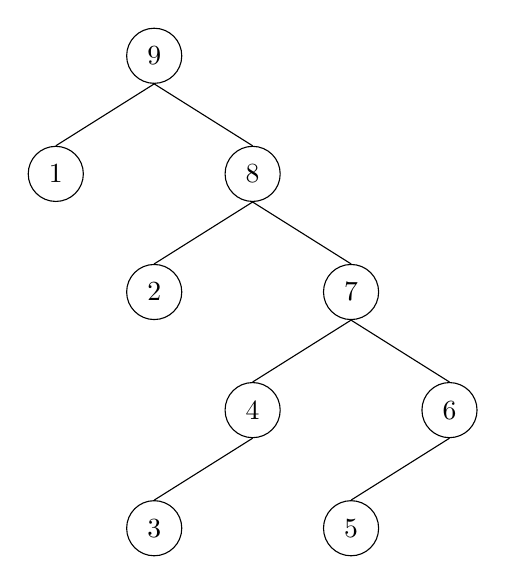
\begin{tikzpicture}[level distance=1.5cm, sibling distance=2.5cm,
  every node/.style={circle, draw, minimum size=0.7cm, inner sep=0}]
  
  \node {9}
    child {node {1}}
    child {node {8}
      child {node {2}}
      child {node {7}
        child {node {4}
          child {node {3}}
          child[missing] {}
        }
        child {node {6}
          child {node {5}}
          child[missing] {}
        }
      }
    };
\end{tikzpicture}


\end{document}